% Created 2019-05-22 mié 14:28
% Intended LaTeX compiler: pdflatex
\documentclass[xcolor={usenames,svgnames,dvipsnames}]{beamer}
\usepackage[utf8]{inputenc}
\usepackage[T1]{fontenc}
\usepackage{graphicx}
\usepackage{grffile}
\usepackage{longtable}
\usepackage{wrapfig}
\usepackage{rotating}
\usepackage[normalem]{ulem}
\usepackage{amsmath}
\usepackage{textcomp}
\usepackage{amssymb}
\usepackage{capt-of}
\usepackage{hyperref}
\usepackage{color}
\usepackage{listings}
\usepackage[spanish]{babel}
\setbeamercolor{alerted text}{fg=Blue}
\setbeamerfont{alerted text}{series=\bfseries}
\setbeamercolor{block title}{bg=structure.fg!20!bg!50!bg}
\setbeamercolor{block body}{use=block title,bg=block title.bg}
\AtBeginSubsection[]{\begin{frame}[plain]\tableofcontents[currentsubsection,sectionstyle=show/shaded,subsectionstyle=show/shaded/hide]\end{frame}}
\AtBeginSection[]{\begin{frame}[plain]\tableofcontents[currentsection,hideallsubsections]\end{frame}}
\lstset{keywordstyle=\color{blue}, commentstyle=\color{gray!90}, basicstyle=\ttfamily\small, columns=fullflexible, breaklines=true,linewidth=\textwidth, backgroundcolor=\color{gray!23}, basewidth={0.5em,0.4em}, literate={á}{{\'a}}1 {ñ}{{\~n}}1 {é}{{\'e}}1 {ó}{{\'o}}1 {º}{{\textordmasculine}}1, showstringspaces=false}
\usepackage{mathpazo}
\hypersetup{colorlinks=true, linkcolor=Blue, urlcolor=Blue}
\usepackage{fancyvrb}
\DefineVerbatimEnvironment{verbatim}{Verbatim}{fontsize=\tiny, formatcom = {\color{black!70}}}
\beamertemplatenavigationsymbolsempty
\setbeamertemplate{footline}[frame number]
\usetheme{Boadilla}
\usecolortheme{rose}
\usefonttheme{serif}
\author{Oscar Perpiñán Lamigueiro \\ \url{http://oscarperpinan.github.io}}
\date{}
\title{Clases y Métodos}
\hypersetup{
 pdfauthor={Oscar Perpiñán Lamigueiro \\ \url{http://oscarperpinan.github.io}},
 pdftitle={Clases y Métodos},
 pdfkeywords={},
 pdfsubject={},
 pdfcreator={Emacs 26.1 (Org mode 9.2)}, 
 pdflang={Spanish}}
\begin{document}

\maketitle

\section{OOP en R}
\label{sec:org9268598}

\begin{frame}[label={sec:org32f0a51}]{Programación Orientada a Objetos (OOP)}
\begin{itemize}
\item Los objetos encapsulan información y control de su comportamiento (\emph{objects}).
\item Las clases describen propiedades de un grupo de objetos (\emph{class}).
\item Se pueden definir clases a partir de otras (\emph{inheritance}).
\item Una función genérica se comporta de forma diferente atendiendo a la
clase de uno (o varios) de sus argumentos (\emph{polymorphism}).
\end{itemize}
\end{frame}
\begin{frame}[label={sec:org315da08},fragile]{OOP en R}
 En \texttt{R} coexisten dos implementaciones de la OOP:
\begin{itemize}
\item \texttt{S3}: elaboración informal con enfasis en las funciones genéricas y el polimorfismo.
\item \texttt{S4}: elaboración formal de clases y métodos.
\end{itemize}
\end{frame}
\begin{frame}[label={sec:orga14bb6f}]{OOP en R}
\begin{block}{Referencias}
\begin{center}
\begin{itemize}
\item \href{http://www.springer.com/gb/book/9780387759357}{Software for Data Analysis}
\item \href{http://developer.r-project.org/howMethodsWork.pdf}{How Methods Work}
\item \href{http://www.stat.auckland.ac.nz/S-Workshop/Gentleman/S4Objects.pdf}{S4 classes in 15 pages}
\item \href{http://bioconductor.org/help/publications/books/r-programming-for-bioinformatics/}{R Programming for Bioinformatics }
\item \href{http://bioconductor.org/help/course-materials/2010/AdvancedR/S4InBioconductor.pdf}{S4 System Development in Bioconductor}
\end{itemize}
\end{center}
\end{block}
\end{frame}

\section{Clases y métodos S3}
\label{sec:orga146f6c}

\subsection{Clases}
\label{sec:org7a7a4a6}
\begin{frame}[label={sec:orgfa1831a},fragile]{Clases}
 Los objetos básicos en \texttt{R} tienen una clase implícita definida en \texttt{S3}. Es accesible con \texttt{class}.
\lstset{language=r,label= ,caption= ,captionpos=b,numbers=none}
\begin{lstlisting}
  x <- rnorm(10)
  class(x)
\end{lstlisting}

\begin{verbatim}
[1] "numeric"
\end{verbatim}


Pero no tienen atributo\ldots{}
\lstset{language=r,label= ,caption= ,captionpos=b,numbers=none}
\begin{lstlisting}
attr(x, 'class')
\end{lstlisting}

\begin{verbatim}
NULL
\end{verbatim}


\ldots{}ni se consideran formalmente objetos
\lstset{language=r,label= ,caption= ,captionpos=b,numbers=none}
\begin{lstlisting}
is.object(x)
\end{lstlisting}

\begin{verbatim}
[1] FALSE
\end{verbatim}
\end{frame}


\begin{frame}[label={sec:orgd6e7369},fragile]{Clases}
 Se puede redefinir la clase de un objecto \texttt{S3} con \texttt{class}
\lstset{language=r,label= ,caption= ,captionpos=b,numbers=none}
\begin{lstlisting}
  class(x) <- 'myNumeric'
  class(x)
\end{lstlisting}

\begin{verbatim}
[1] "myNumeric"
\end{verbatim}


Ahora sí es un objeto\ldots{} 
\lstset{language=r,label= ,caption= ,captionpos=b,numbers=none}
\begin{lstlisting}
is.object(x)
\end{lstlisting}

\begin{verbatim}
[1] TRUE
\end{verbatim}


y su atributo está definido
\lstset{language=r,label= ,caption= ,captionpos=b,numbers=none}
\begin{lstlisting}
attr(x, 'class')
\end{lstlisting}

\begin{verbatim}
[1] "myNumeric"
\end{verbatim}


Sin embargo, su modo de almacenamiento (\emph{clase intrínseca}) no cambia:
\lstset{language=r,label= ,caption= ,captionpos=b,numbers=none}
\begin{lstlisting}
  mode(x)
\end{lstlisting}

\begin{verbatim}
[1] "numeric"
\end{verbatim}
\end{frame}

\begin{frame}[label={sec:org4d90674},fragile]{Definición de Clases}
 \lstset{language=r,label= ,caption= ,captionpos=b,numbers=none}
\begin{lstlisting}
  task1 <- list(what='Write an email',
                when=as.Date('2013-01-01'),
                priority='Low')
  class(task1) <- 'Task'
  task1
\end{lstlisting}

\begin{verbatim}
$what
[1] "Write an email"

$when
[1] "2013-01-01"

$priority
[1] "Low"

attr(,"class")
[1] "Task"
\end{verbatim}

\lstset{language=r,label= ,caption= ,captionpos=b,numbers=none}
\begin{lstlisting}
  task2 <- list(what='Find and fix bugs',
                when=as.Date('2013-03-15'),
                priority='High')
  class(task2) <- 'Task'
\end{lstlisting}
\end{frame}

\begin{frame}[label={sec:orgd0d65e6},fragile]{Definición de Clases}
 \lstset{language=r,label= ,caption= ,captionpos=b,numbers=none}
\begin{lstlisting}
  myToDo <- list(task1, task2)
  class(myToDo) <- c('ToDo3')
  myToDo
\end{lstlisting}

\begin{verbatim}
[[1]]
$what
[1] "Write an email"

$when
[1] "2013-01-01"

$priority
[1] "Low"

attr(,"class")
[1] "Task"

[[2]]
$what
[1] "Find and fix bugs"

$when
[1] "2013-03-15"

$priority
[1] "High"

attr(,"class")
[1] "Task"

attr(,"class")
[1] "ToDo3"
\end{verbatim}
\end{frame}

\begin{frame}[label={sec:orgf159753},fragile]{Problemas de la sencillez de \texttt{S3}}
 \lstset{language=r,label= ,caption= ,captionpos=b,numbers=none}
\begin{lstlisting}
  notToDo <- list(task1, 2019)
  class(notToDo) <- c('ToDo3')
  notToDo
\end{lstlisting}

\begin{verbatim}
[[1]]
$what
[1] "Write an email"

$when
[1] "2013-01-01"

$priority
[1] "Low"

attr(,"class")
[1] "Task"

[[2]]
[1] 2019

attr(,"class")
[1] "ToDo3"
\end{verbatim}
\end{frame}

\subsection{Métodos}
\label{sec:org2c4d0fc}
\begin{frame}[label={sec:org4c6376d},fragile]{Métodos con \texttt{S3}}
 Son \alert{sencillos} de usar e implementar pero \alert{poco robustos}.

Se definen a partir de un método genérico\ldots{}
\lstset{language=r,label= ,caption= ,captionpos=b,numbers=none}
\begin{lstlisting}
summary
\end{lstlisting}

\begin{verbatim}
function (object, ...) 
UseMethod("summary")
<bytecode: 0x5590c6b26c38>
<environment: namespace:base>
\end{verbatim}


\ldots{}añadiendo a la función el nombre de la clase con un punto como separador. 
\lstset{language=r,label= ,caption= ,captionpos=b,numbers=none}
\begin{lstlisting}
summary.data.frame
\end{lstlisting}

\begin{verbatim}
function (object, maxsum = 7L, digits = max(3L, getOption("digits") - 
    3L), ...) 
{
    ncw <- function(x) {
        z <- nchar(x, type = "w")
        if (any(na <- is.na(z))) {
            z[na] <- nchar(encodeString(z[na]), "b")
        }
        z
    }
    z <- lapply(X = as.list(object), FUN = summary, maxsum = maxsum, 
        digits = 12L, ...)
    nv <- length(object)
    nm <- names(object)
    lw <- numeric(nv)
    nr <- if (nv) 
        max(vapply(z, function(x) NROW(x) + !is.null(attr(x, 
            "NAs")), integer(1)))
    else 0
    for (i in seq_len(nv)) {
        sms <- z[[i]]
        if (is.matrix(sms)) {
            cn <- paste(nm[i], gsub("^ +", "", colnames(sms), 
                useBytes = TRUE), sep = ".")
            tmp <- format(sms)
            if (nrow(sms) < nr) 
                tmp <- rbind(tmp, matrix("", nr - nrow(sms), 
                  ncol(sms)))
            sms <- apply(tmp, 1L, function(x) paste(x, collapse = "  "))
            wid <- sapply(tmp[1L, ], nchar, type = "w")
            blanks <- paste(character(max(wid)), collapse = " ")
            wcn <- ncw(cn)
            pad0 <- floor((wid - wcn)/2)
            pad1 <- wid - wcn - pad0
            cn <- paste0(substring(blanks, 1L, pad0), cn, substring(blanks, 
                1L, pad1))
            nm[i] <- paste(cn, collapse = "  ")
        }
        else {
            sms <- format(sms, digits = digits)
            lbs <- format(names(sms))
            sms <- paste0(lbs, ":", sms, "  ")
            lw[i] <- ncw(lbs[1L])
            length(sms) <- nr
        }
        z[[i]] <- sms
    }
    if (nv) {
        z <- unlist(z, use.names = TRUE)
        dim(z) <- c(nr, nv)
        if (anyNA(lw)) 
            warning("probably wrong encoding in names(.) of column ", 
                paste(which(is.na(lw)), collapse = ", "))
        blanks <- paste(character(max(lw, na.rm = TRUE) + 2L), 
            collapse = " ")
        pad <- floor(lw - ncw(nm)/2)
        nm <- paste0(substring(blanks, 1, pad), nm)
        dimnames(z) <- list(rep.int("", nr), nm)
    }
    else {
        z <- character()
        dim(z) <- c(nr, nv)
    }
    attr(z, "class") <- c("table")
    z
}
<bytecode: 0x5590c723a6b8>
<environment: namespace:base>
\end{verbatim}
\end{frame}

\begin{frame}[label={sec:org6209a40},fragile]{Métodos con \texttt{S3}}
 Con \texttt{methods} podemos averiguar los métodos que hay definidos para una función particular:
\lstset{language=r,label= ,caption= ,captionpos=b,numbers=none}
\begin{lstlisting}
methods('summary')
\end{lstlisting}

\begin{verbatim}
 [1] summary.aov                    summary.aovlist*              
 [3] summary.aspell*                summary.check_packages_in_dir*
 [5] summary.connection             summary.data.frame            
 [7] summary.Date                   summary.default               
 [9] summary.ecdf*                  summary.factor                
[11] summary.glm                    summary.infl*                 
[13] summary.lm                     summary.loess*                
[15] summary.manova                 summary.matrix                
[17] summary.mlm*                   summary.nls*                  
[19] summary.packageStatus*         summary.PDF_Dictionary*       
[21] summary.PDF_Stream*            summary.POSIXct               
[23] summary.POSIXlt                summary.ppr*                  
[25] summary.prcomp*                summary.princomp*             
[27] summary.proc_time              summary.shingle*              
[29] summary.srcfile                summary.srcref                
[31] summary.stepfun                summary.stl*                  
[33] summary.table                  summary.trellis*              
[35] summary.tukeysmooth*           summary.warnings              
see '?methods' for accessing help and source code
\end{verbatim}
\end{frame}

\begin{frame}[label={sec:org9fb195a},fragile]{Métodos con \texttt{S3}}
 Si no hay un método definido para la clase del objeto, \texttt{UseMethod} ejecuta la función por defecto:
\lstset{language=r,label= ,caption= ,captionpos=b,numbers=none}
\begin{lstlisting}
summary.default
\end{lstlisting}

\begin{verbatim}
function (object, ..., digits) 
{
    if (is.factor(object)) 
        return(summary.factor(object, ...))
    else if (is.matrix(object)) {
        if (missing(digits)) 
            return(summary.matrix(object, ...))
        else return(summary.matrix(object, digits = digits, ...))
    }
    value <- if (is.logical(object)) 
        c(Mode = "logical", {
            tb <- table(object, exclude = NULL, useNA = "ifany")
            if (!is.null(n <- dimnames(tb)[[1L]]) && any(iN <- is.na(n))) dimnames(tb)[[1L]][iN] <- "NA's"
            tb
        })
    else if (is.numeric(object)) {
        nas <- is.na(object)
        object <- object[!nas]
        qq <- stats::quantile(object)
        qq <- c(qq[1L:3L], mean(object), qq[4L:5L])
        if (!missing(digits)) 
            qq <- signif(qq, digits)
        names(qq) <- c("Min.", "1st Qu.", "Median", "Mean", "3rd Qu.", 
            "Max.")
        if (any(nas)) 
            c(qq, `NA's` = sum(nas))
        else qq
    }
    else if (is.recursive(object) && !is.language(object) && 
        (n <- length(object))) {
        sumry <- array("", c(n, 3L), list(names(object), c("Length", 
            "Class", "Mode")))
        ll <- numeric(n)
        for (i in 1L:n) {
            ii <- object[[i]]
            ll[i] <- length(ii)
            cls <- oldClass(ii)
            sumry[i, 2L] <- if (length(cls)) 
                cls[1L]
            else "-none-"
            sumry[i, 3L] <- mode(ii)
        }
        sumry[, 1L] <- format(as.integer(ll))
        sumry
    }
    else c(Length = length(object), Class = class(object), Mode = mode(object))
    class(value) <- c("summaryDefault", "table")
    value
}
<bytecode: 0x5590c6b296b8>
<environment: namespace:base>
\end{verbatim}
\end{frame}

\begin{frame}[label={sec:orge9a80bb},fragile]{Ejemplo de definición de método genérico}
 En primer lugar, definimos la función con \texttt{UseMethod}:
\lstset{language=r,label= ,caption= ,captionpos=b,numbers=none}
\begin{lstlisting}
  myFun <- function(x, ...)UseMethod('myFun')
\end{lstlisting}

\ldots{} y la función por defecto.
\lstset{language=r,label= ,caption= ,captionpos=b,numbers=none}
\begin{lstlisting}
  myFun.default <- function(x, ...){
    cat('Funcion genérica\n')
    print(x)
    }
\end{lstlisting}
\end{frame}

\begin{frame}[label={sec:org92bd248},fragile]{Ejemplo de definición de método genérico}
 Dado que aún no hay métodos definidos, esta función ejecutará la función por defecto.
\lstset{language=r,label= ,caption= ,captionpos=b,numbers=none}
\begin{lstlisting}
methods('myFun')
\end{lstlisting}

\begin{verbatim}
[1] myFun.default
see '?methods' for accessing help and source code
\end{verbatim}


\lstset{language=r,label= ,caption= ,captionpos=b,numbers=none}
\begin{lstlisting}
x <- rnorm(10)
myFun(x)
\end{lstlisting}

\begin{verbatim}
Funcion genérica
 [1] -0.69530828 -0.86033073  0.46258729  0.09141196  0.87631683  1.09642821
 [7]  1.78801672  1.11956120  0.11451895  0.96900200
\end{verbatim}


\lstset{language=r,label= ,caption= ,captionpos=b,numbers=none}
\begin{lstlisting}
myFun(task1)
\end{lstlisting}

\begin{verbatim}
Funcion genérica
$what
[1] "Write an email"

$when
[1] "2013-01-01"

$priority
[1] "Low"

attr(,"class")
[1] "Task"
\end{verbatim}
\end{frame}


\begin{frame}[label={sec:orga8120af},fragile]{Ejemplo de definición de método específico}
 \lstset{language=r,label= ,caption= ,captionpos=b,numbers=none}
\begin{lstlisting}
myFun.Task <- function(x, number,...)
{
    if (!missing(number))
        cat('Task no.', number,':\n')
    cat('What: ', x$what,
        '- When:', as.character(x$when),
        '- Priority:', x$priority,
        '\n')
}
\end{lstlisting}

\lstset{language=r,label= ,caption= ,captionpos=b,numbers=none}
\begin{lstlisting}
methods(myFun)
\end{lstlisting}

\begin{verbatim}
[1] myFun.default myFun.Task   
see '?methods' for accessing help and source code
\end{verbatim}


\lstset{language=r,label= ,caption= ,captionpos=b,numbers=none}
\begin{lstlisting}
methods(class='Task')
\end{lstlisting}

\begin{verbatim}
[1] myFun
see '?methods' for accessing help and source code
\end{verbatim}
\end{frame}

\begin{frame}[label={sec:org44e8a52},fragile]{Método de \texttt{Task}}
 \lstset{language=r,label= ,caption= ,captionpos=b,numbers=none}
\begin{lstlisting}
myFun(task1)
\end{lstlisting}

\begin{verbatim}
What:  Write an email - When: 2013-01-01 - Priority: Low
\end{verbatim}


\lstset{language=r,label= ,caption= ,captionpos=b,numbers=none}
\begin{lstlisting}
myFun(task2)
\end{lstlisting}

\begin{verbatim}
What:  Find and fix bugs - When: 2013-03-15 - Priority: High
\end{verbatim}


\lstset{language=r,label= ,caption= ,captionpos=b,numbers=none}
\begin{lstlisting}
myFun(myToDo)
\end{lstlisting}

\begin{verbatim}
Funcion genérica
[[1]]
$what
[1] "Write an email"

$when
[1] "2013-01-01"

$priority
[1] "Low"

attr(,"class")
[1] "Task"

[[2]]
$what
[1] "Find and fix bugs"

$when
[1] "2013-03-15"

$priority
[1] "High"

attr(,"class")
[1] "Task"

attr(,"class")
[1] "ToDo3"
\end{verbatim}
\end{frame}

\begin{frame}[label={sec:org8f8e755},fragile]{Definición del método para \texttt{ToDo3}}
 \begin{block}{Ejercicio}
Define un método de \texttt{myFun} para la clase \texttt{ToDo3} con dos enfoques: sin tener en cuenta el método definido para \texttt{Task}; teniendo en cuenta el método para \texttt{Task}.
\end{block}
\end{frame}


\begin{frame}[label={sec:orge4a58c0},fragile]{Definición del método para \texttt{ToDo3}}
 \lstset{language=r,label= ,caption= ,captionpos=b,numbers=none}
\begin{lstlisting}
  myFun.ToDo3 <- function(x, ...){
      cat('This is my ToDo list:\n')
      ## Cada uno de los elementos de un
      ## objeto ToDo3 son Task.  Por tanto,
      ## x[[i]] es de clase Task y
      ## print(x[[i]]) ejecuta el metodo
      ## print.Task
    for (i in seq_along(x)) myFun(x[[i]], i)
      cat('--------------------\n')
  }
\end{lstlisting}

\lstset{language=r,label= ,caption= ,captionpos=b,numbers=none}
\begin{lstlisting}
myFun(myToDo)
\end{lstlisting}

\begin{verbatim}
This is my ToDo list:
Task no. 1 :
What:  Write an email - When: 2013-01-01 - Priority: Low 
Task no. 2 :
What:  Find and fix bugs - When: 2013-03-15 - Priority: High 
--------------------
\end{verbatim}
\end{frame}


\section{Clases y métodos S4}
\label{sec:orgb39583d}

\subsection{Clases en \texttt{S4}}
\label{sec:orga00987b}
\begin{frame}[label={sec:org014bd51},fragile]{Clases en \texttt{S4}}
 Se construyen con \texttt{setClass}, que acepta varios argumentos
\begin{itemize}
\item \texttt{Class}: nombre de la clase.
\item \texttt{slots}: una lista con las clases de cada componente. Los nombres de este vector corresponden a los nombres de los componentes (\texttt{slot}).
\item \texttt{contains}: un vector con las clases que esta nueva clase extiende.
\item \texttt{prototype}: un objeto proporcionando el contenido por defecto para los componentes definidos en \texttt{slots}.
\item \texttt{validity}: a función que comprueba la validez de la clase creada con la información suministrada.
\end{itemize}
\end{frame}

\begin{frame}[label={sec:org2dbb86f}]{Datos de ejemplo}
Vamos a ilustrar esta sección con datos de seguimiento GPS de gaviotas\footnote{\url{https://lifewatch.inbo.be/blog/posts/bird-tracking-data-published.html}} empleando un extracto del conjunto de datos\footnote{\url{https://lifewatch.inbo.be/blog/files/bird\_tracking.zip}}.
\begin{center}
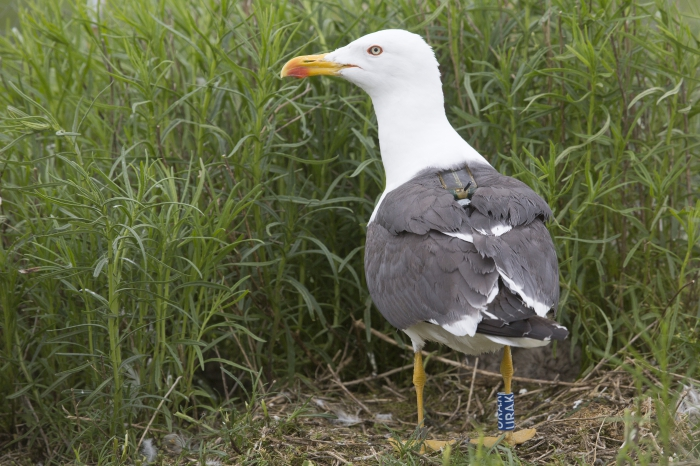
\includegraphics[height=0.5\textheight]{figs/73915_lesser-black-backed-gull-with-transmitter.jpg}
\end{center}
\end{frame}

\begin{frame}[label={sec:orgfb3c3e4},fragile]{Definición de una nueva clase}
 \lstset{language=r,label= ,caption= ,captionpos=b,numbers=none}
\begin{lstlisting}
setClass('bird',
         slots = c(
             name = 'character',
             lat = 'numeric',
             lon = 'numeric',
             alt = 'numeric',
             speed = 'numeric',
             time = 'POSIXct')
         )
\end{lstlisting}
\end{frame}

\begin{frame}[label={sec:orgff3f4c5},fragile]{Funciones para obtener información de una clase}
 \lstset{language=r,label= ,caption= ,captionpos=b,numbers=none}
\begin{lstlisting}
getClass('bird')
\end{lstlisting}

\begin{verbatim}
Class "bird" [in ".GlobalEnv"]

Slots:
                                                                  
Name:       name       lat       lon       alt     speed      time
Class: character   numeric   numeric   numeric   numeric   POSIXct
\end{verbatim}


\lstset{language=r,label= ,caption= ,captionpos=b,numbers=none}
\begin{lstlisting}
getSlots('bird')
\end{lstlisting}

\begin{verbatim}
       name         lat         lon         alt       speed        time 
"character"   "numeric"   "numeric"   "numeric"   "numeric"   "POSIXct"
\end{verbatim}


\lstset{language=r,label= ,caption= ,captionpos=b,numbers=none}
\begin{lstlisting}
slotNames('bird')
\end{lstlisting}

\begin{verbatim}
[1] "name"  "lat"   "lon"   "alt"   "speed" "time"
\end{verbatim}
\end{frame}

\begin{frame}[label={sec:orgbb30588},fragile]{Creación de un objeto con la clase definida}
 Una vez que la clase ha sido definida con \texttt{setClass}, se puede crear un objeto nuevo con \texttt{new}. Es habitual definir funciones que construyen y modifican objetos para evitar el uso directo de \texttt{new}:
\lstset{language=r,label= ,caption= ,captionpos=b,numbers=none}
\begin{lstlisting}
readBird <- function(name, path)
{
    csvFile <- file.path(path, paste0(name, ".csv"))

    vals <- read.csv(csvFile)
    
    new('bird',
        name = name,
        lat = vals$latitude,
        lon = vals$longitude,
        alt = vals$altitude,
        speed = vals$speed_2d,
        time = as.POSIXct(vals$date_time)
        )
}  
\end{lstlisting}
\end{frame}

\begin{frame}[label={sec:orgb9a713a},fragile]{Creación de objetos con la clase definida}
 \lstset{language=r,label= ,caption= ,captionpos=b,numbers=none}
\begin{lstlisting}
eric <- readBird("eric", "data")
nico <- readBird("nico", "data")
sanne <- readBird("sanne", "data")
\end{lstlisting}
\end{frame}


\begin{frame}[label={sec:org1cd7eef},fragile]{Acceso a los slots}
 A diferencia de \texttt{\$} en listas y \texttt{data.frame}, para extraer información de los \emph{slots} hay que emplear \texttt{@} (pero no es recomendable):
\lstset{language=r,label= ,caption= ,captionpos=b,numbers=none}
\begin{lstlisting}
eric@name
\end{lstlisting}

\begin{verbatim}
[1] "eric"
\end{verbatim}


\lstset{language=r,label= ,caption= ,captionpos=b,numbers=none}
\begin{lstlisting}
summary(eric@speed)
\end{lstlisting}

\begin{verbatim}
  Min. 1st Qu.  Median    Mean 3rd Qu.    Max.    NA's 
0.0000  0.3437  1.0031  2.3005  2.4792 63.4881      85
\end{verbatim}
\end{frame}

\begin{frame}[label={sec:orgfd46b3b},fragile]{Clases \texttt{S4} con slots tipo lista}
 \lstset{language=r,label= ,caption= ,captionpos=b,numbers=none}
\begin{lstlisting}
setClass("flock",
         slots = c(
             name = "character",
             members = "list")
         )

\end{lstlisting}

\lstset{language=r,label= ,caption= ,captionpos=b,numbers=none}
\begin{lstlisting}
notAFlock <- new("flock",
                 name = "flock0",
                 members = list(eric,
                                3,
                                "hello"))
sapply(notAFlock@members, class)
\end{lstlisting}

\begin{verbatim}
[1] "bird"      "numeric"   "character"
\end{verbatim}
\end{frame}

\begin{frame}[label={sec:org0ca83fc},fragile]{Función de validación}
 \lstset{language=r,label= ,caption= ,captionpos=b,numbers=none}
\begin{lstlisting}
valida <- function (object) {
    if (any(sapply(object@members,
                   function(x) !is(x, "bird")))) 
        stop("only bird objects are accepted.")
    return(TRUE)
}

setClass("flock",
         slots = c(
             name = "character",
             members = "list"),
         validity = valida
         )
\end{lstlisting}
\end{frame}

\begin{frame}[label={sec:org8576ba5},fragile]{Ejemplo de objeto \texttt{S4} con slot tipo \texttt{list}}
 \lstset{language=r,label= ,caption= ,captionpos=b,numbers=none}
\begin{lstlisting}
newFlock <- function(name, ...){
    birds <- list(...)
    new("flock",
        name = name,
        members = birds)
}
\end{lstlisting}

\lstset{language=r,label= ,caption= ,captionpos=b,numbers=none}
\begin{lstlisting}
notAFlock <- newFlock("flock0",
                    eric, 2, "hello")
\end{lstlisting}

\begin{verbatim}
Error in validityMethod(object) : only bird objects are accepted.
\end{verbatim}


\lstset{language=r,label= ,caption= ,captionpos=b,numbers=none}
\begin{lstlisting}
myFlock <- newFlock("flock1",
                    eric, nico, sanne)
\end{lstlisting}
\end{frame}

\subsection{Métodos en \texttt{S4}}
\label{sec:orgb58d5fe}

\begin{frame}[label={sec:orgdc429e9},fragile]{Métodos en \texttt{S4}: \texttt{setMethod}}
 \begin{itemize}
\item Normalmente se definen con \texttt{setMethod} suministrando:
\begin{itemize}
\item la clase de los objetos para \emph{esta} definición del
método (\texttt{signature})
\item la función a ejecutar (\texttt{definition}).
\end{itemize}
\end{itemize}
\lstset{language=r,label= ,caption= ,captionpos=b,numbers=none}
\begin{lstlisting}
setMethod('show',
          signature = "bird",
          definition = function(object)
          {
              cat("Name: ", object@name, "\n")
              cat("Latitude: ", summary(object@lat), "\n")
              cat("Longitude: ", summary(object@lon), "\n")
              cat("Speed: ", summary(object@speed), "\n")
          })
\end{lstlisting}

\lstset{language=r,label= ,caption= ,captionpos=b,numbers=none}
\begin{lstlisting}
eric
\end{lstlisting}

\begin{verbatim}
Name:  eric 
Latitude:  30.17401 30.43032 30.4624 39.05512 50.11692 51.36129 
Longitude:  -9.928351 -9.643971 -9.630419 -4.409152 2.65808 3.601085 
Speed:  0 0.3436568 1.00312 2.300545 2.479153 63.48807 85
\end{verbatim}
\end{frame}

\begin{frame}[label={sec:orgfac9ba4},fragile]{Métodos en \texttt{S4}: \texttt{setMethod}}
 \lstset{language=r,label= ,caption= ,captionpos=b,numbers=none}
\begin{lstlisting}
setMethod('show',
          signature = "flock",
          definition = function(object)
          {
              cat("Flock Name: ", object@name, "\n")
              N <- length(object@members)
              lapply(seq_len(N), function(i)
              {
                  cat("Bird #", i, "\n")
                  print(object@members[[i]])
              })
          })
\end{lstlisting}

\lstset{language=r,label= ,caption= ,captionpos=b,numbers=none}
\begin{lstlisting}
myFlock
\end{lstlisting}

\begin{verbatim}
Flock Name:  flock1 
Bird # 1 
Name:  eric 
Latitude:  30.17401 30.43032 30.4624 39.05512 50.11692 51.36129 
Longitude:  -9.928351 -9.643971 -9.630419 -4.409152 2.65808 3.601085 
Speed:  0 0.3436568 1.00312 2.300545 2.479153 63.48807 85 
Bird # 2 
Name:  nico 
Latitude:  12.35442 15.89667 23.82977 31.08407 50.21611 51.51845 
Longitude:  -17.62615 -16.75806 -15.94404 -8.311241 3.609543 4.857561 
Speed:  0 0.4876218 1.541914 2.908726 3.717069 48.38151 113 
Bird # 3 
Name:  sanne 
Latitude:  13.88409 14.09925 14.50451 21.04743 22.94247 51.37478 
Longitude:  -17.37979 -16.81003 -16.75907 -13.88172 -16.0166 3.389886 
Speed:  0 0.4049691 1.1456 2.450434 2.869024 57.20175 245
\end{verbatim}
\end{frame}

\begin{frame}[label={sec:org03e470e},fragile]{Métodos en \texttt{S4}: \texttt{setGeneric}}
 \begin{itemize}
\item Es necesario que exista un método genérico ya definido.
\end{itemize}
\lstset{language=r,label= ,caption= ,captionpos=b,numbers=none}
\begin{lstlisting}
isGeneric("as.data.frame")
\end{lstlisting}

\begin{verbatim}
[1] FALSE
\end{verbatim}


\begin{itemize}
\item Si no existe, se define con \texttt{setGeneric} (y quizás \texttt{standardGeneric}).
\end{itemize}
\lstset{language=r,label= ,caption= ,captionpos=b,numbers=none}
\begin{lstlisting}
setGeneric("as.data.frame")
\end{lstlisting}

\begin{verbatim}
[1] "as.data.frame"
\end{verbatim}


\begin{itemize}
\item La función \texttt{definition} debe respetar los argumentos de la función genérica y en el mismo orden.
\end{itemize}
\lstset{language=r,label= ,caption= ,captionpos=b,numbers=none}
\begin{lstlisting}
getGeneric("as.data.frame")
\end{lstlisting}

\begin{verbatim}
standardGeneric for "as.data.frame" defined from package "base"

function (x, row.names = NULL, optional = FALSE, ...) 
standardGeneric("as.data.frame")
<environment: 0x5590c6356310>
Methods may be defined for arguments: x, row.names, optional
Use  showMethods("as.data.frame")  for currently available ones.
\end{verbatim}
\end{frame}


\begin{frame}[label={sec:orgd501e67},fragile]{Métodos en \texttt{S4}: ejemplo con \texttt{as.data.frame}}
 \lstset{language=r,label= ,caption= ,captionpos=b,numbers=none}
\begin{lstlisting}
setMethod("as.data.frame",
          signature = "bird",
          definition = function(x, ...)
          {
              data.frame(
                  name = x@name,
                  lat = x@lat,
                  lon = x@lon,
                  alt = x@alt,
                  speed = x@speed,
                  time = x@time)
          })
\end{lstlisting}

\lstset{language=r,label= ,caption= ,captionpos=b,numbers=none}
\begin{lstlisting}
ericDF <- as.data.frame(eric)
\end{lstlisting}
\end{frame}

\begin{frame}[label={sec:org24b2d45},fragile]{Métodos en \texttt{S4}: ejemplo con \texttt{as.data.frame}}
 \begin{block}{Ejercicio}
Define un método de \texttt{as.data.frame} para la clase \texttt{flock} a partir del método para la clase \texttt{bird}.
\end{block}
\end{frame}

\begin{frame}[label={sec:orgb830977},fragile]{Métodos en \texttt{S4}: ejemplo con \texttt{as.data.frame}}
 \lstset{language=r,label= ,caption= ,captionpos=b,numbers=none}
\begin{lstlisting}
setMethod("as.data.frame",
          signature = "flock",
          definition = function(x, ...)
          {
              dfs <- lapply(x@members, as.data.frame)
              dfs <- do.call(rbind, dfs)
              dfs$flock_name <- x@name
              dfs
          })
\end{lstlisting}

\lstset{language=r,label= ,caption= ,captionpos=b,numbers=none}
\begin{lstlisting}
flockDF <- as.data.frame(myFlock)
\end{lstlisting}
\end{frame}

\begin{frame}[label={sec:orgfc37420},fragile]{Métodos en \texttt{S4}: ejemplo con \texttt{xyplot}}
 \lstset{language=r,label= ,caption= ,captionpos=b,numbers=none}
\begin{lstlisting}
library(lattice)

setGeneric("xyplot")

setMethod('xyplot',
          signature = "bird",
          definition = function(x, data = NULL, ...)
          {
              df <- as.data.frame(x)
              xyplot(lat ~ lon, data = df, ...)
          })    
\end{lstlisting}

\begin{verbatim}
[1] "xyplot"
\end{verbatim}


\lstset{language=r,label= ,caption= ,captionpos=b,numbers=none}
\begin{lstlisting}
xyplot(eric)
\end{lstlisting}
\end{frame}


\begin{frame}[label={sec:org5828ac7},fragile]{Métodos en \texttt{S4}: ejemplo con \texttt{xyplot}}
 \begin{block}{Ejercicio}
Define un método de \texttt{xyplot} para la clase \texttt{bird} que permita elegir entre diferentes modos de representación:
\begin{itemize}
\item \texttt{lontime}
\item \texttt{lattime}
\item \texttt{latlon}
\item \texttt{speed}
\end{itemize}
\end{block}
\end{frame}

\begin{frame}[label={sec:orga80ef18},fragile]{Métodos en \texttt{S4}: ejemplo con \texttt{xyplot}}
 \lstset{language=r,label= ,caption= ,captionpos=b,numbers=none}
\begin{lstlisting}
setMethod('xyplot',
          signature = "bird",
          definition = function(x, data = NULL,
                                mode = "latlon", ...)
          {
              df <- as.data.frame(x)
              switch(mode,
                     lontime = xyplot(lon ~ time, data = df, ...),
                     lattime = xyplot(lat ~ time, data = df, ...),
                     latlon = xyplot(lat ~ lon, data = df, ...),
                     speed = xyplot(speed ~ time, data = df, ...)
                     )
          })    
\end{lstlisting}

\lstset{language=r,label= ,caption= ,captionpos=b,numbers=none}
\begin{lstlisting}
xyplot(eric, mode = "lontime")
\end{lstlisting}
\end{frame}

\begin{frame}[label={sec:org8a3c1b2},fragile]{Métodos en \texttt{S4}: ejemplo con \texttt{xyplot}}
 \begin{block}{Ejercicio}
Define un método de \texttt{xyplot} para la clase \texttt{flock} usando el color para distinguir a los diferentes integrantes (argumento \texttt{group} en \texttt{xyplot}).
\end{block}
\end{frame}

\begin{frame}[label={sec:org60d24f4},fragile]{Métodos en \texttt{S4}: ejemplo con \texttt{xyplot}}
 \lstset{language=r,label= ,caption= ,captionpos=b,numbers=none}
\begin{lstlisting}
setMethod('xyplot',
          signature = "flock",
          definition = function(x, data = NULL, ...)
          {
              df <- as.data.frame(x)
              xyplot(lon ~ lat,
                     group = name,
                     data = df,
                     auto.key = list(space = "right"))
              })
\end{lstlisting}

\lstset{language=r,label= ,caption= ,captionpos=b,numbers=none}
\begin{lstlisting}
xyplot(myFlock)
\end{lstlisting}
\end{frame}

\subsection{Clases \texttt{S3} con clases y métodos \texttt{S4}}
\label{sec:orga24c04d}

\begin{frame}[label={sec:orgbdb936f},fragile]{Clases \texttt{S3} con clases y métodos \texttt{S4}}
 Para usar objetos de clase \texttt{S3} en \texttt{signatures} de métodos \texttt{S4} o
como contenido de \texttt{slots} de una clase \texttt{S4} hay que registrarlos con
\texttt{setOldClass}:
\lstset{language=r,label= ,caption= ,captionpos=b,numbers=none}
\begin{lstlisting}
setOldClass('lm')
\end{lstlisting}

\lstset{language=r,label= ,caption= ,captionpos=b,numbers=none}
\begin{lstlisting}
getClass('lm')
\end{lstlisting}

\begin{verbatim}
Virtual Class "lm" [package "methods"]

Slots:
                
Name:   .S3Class
Class: character

Extends: "oldClass"

Known Subclasses: 
Class "mlm", directly
Class "aov", directly
Class "glm", directly
Class "maov", by class "mlm", distance 2
Class "glm.null", by class "glm", distance 2
\end{verbatim}
\end{frame}

\begin{frame}[label={sec:org785edf4},fragile]{Ejemplo con \texttt{lm} y \texttt{xyplot}}
 Definimos un método genérico para \texttt{xyplot}
\lstset{language=r,label= ,caption= ,captionpos=b,numbers=none}
\begin{lstlisting}
library(lattice)
setGeneric('xyplot')
\end{lstlisting}

\begin{verbatim}
[1] "xyplot"
\end{verbatim}


Definimos un método para la clase \texttt{lm} usando \texttt{xyplot}.
\lstset{language=r,label= ,caption= ,captionpos=b,numbers=none}
\begin{lstlisting}
setMethod('xyplot',
          signature = c(x = 'lm',
                        data = 'missing'),
          definition = function(x, data,
                                ...)
          {
              fitted <- fitted(x)
              residuals <- residuals(x)
              xyplot(residuals ~ fitted,...)
          })

\end{lstlisting}
\end{frame}

\begin{frame}[label={sec:org7de9155},fragile]{Ejemplo con \texttt{lm} y \texttt{xyplot}}
 Recuperamos la regresión que empleamos en el apartado de Estadística:
\lstset{language=r,label= ,caption= ,captionpos=b,numbers=none}
\begin{lstlisting}
lmFertEdu <- lm(Fertility ~ Education, data = swiss)
summary(lmFertEdu)
\end{lstlisting}

\begin{verbatim}

Call:
lm(formula = Fertility ~ Education, data = swiss)

Residuals:
    Min      1Q  Median      3Q     Max 
-17.036  -6.711  -1.011   9.526  19.689 

Coefficients:
            Estimate Std. Error t value Pr(>|t|)    
(Intercept)  79.6101     2.1041  37.836  < 2e-16 ***
Education    -0.8624     0.1448  -5.954 3.66e-07 ***
---
Signif. codes:  0 ‘***’ 0.001 ‘**’ 0.01 ‘*’ 0.05 ‘.’ 0.1 ‘ ’ 1

Residual standard error: 9.446 on 45 degrees of freedom
Multiple R-squared:  0.4406,	Adjusted R-squared:  0.4282 
F-statistic: 35.45 on 1 and 45 DF,  p-value: 3.659e-07
\end{verbatim}
\end{frame}


\begin{frame}[label={sec:orge7bc5e2},fragile]{Ejemplo con \texttt{lm} y \texttt{xyplot}}
 \lstset{language=r,label= ,caption= ,captionpos=b,numbers=none}
\begin{lstlisting}
xyplot(lmFertEdu, col='red', pch = 19,
       type = c('p', 'g'))
\end{lstlisting}
\begin{center}
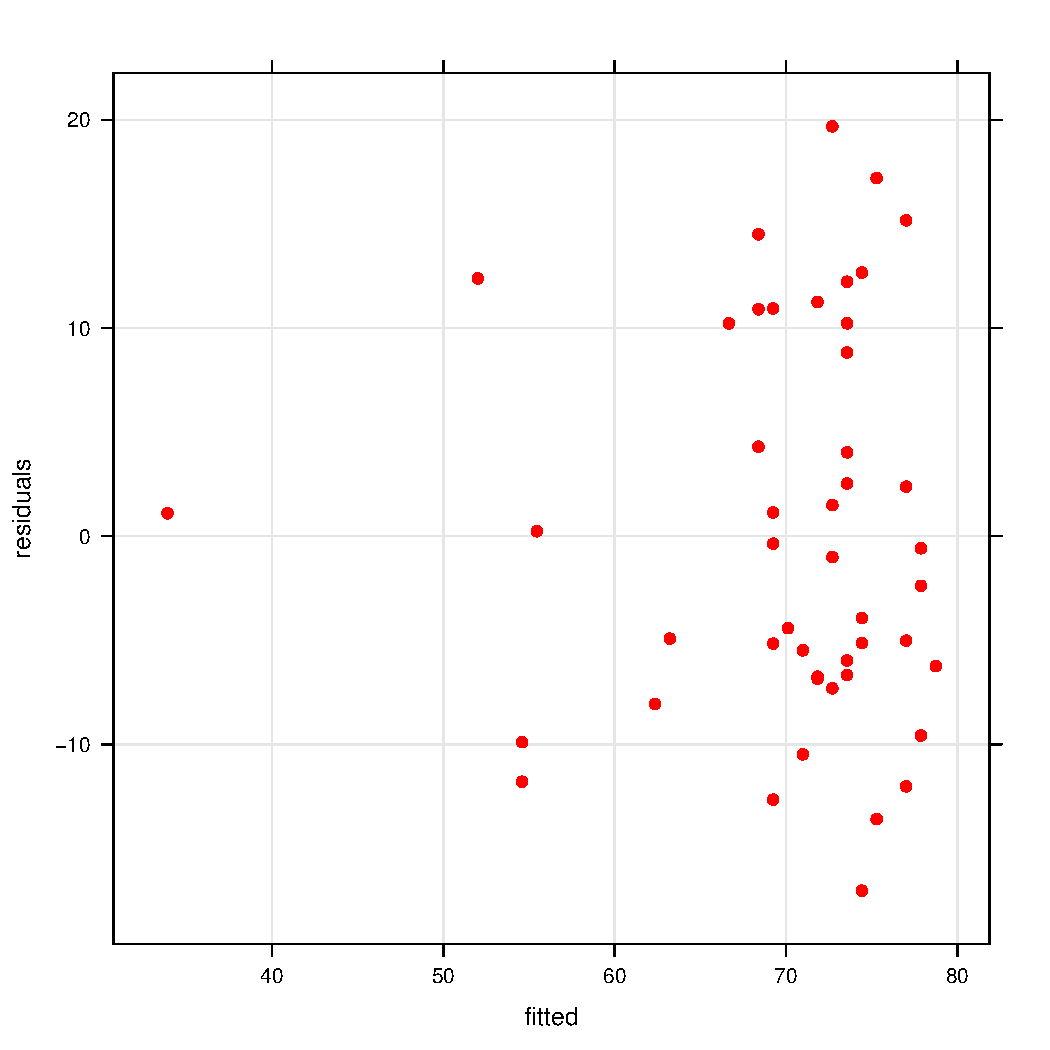
\includegraphics[height=0.7\textheight]{figs/xyplotS4.pdf}
\end{center}
\end{frame}
\end{document}